\documentclass{article}

\usepackage{polski}
\usepackage{polski}
\usepackage{amsmath}
\usepackage{graphicx}
\usepackage{float}
\usepackage{subfig}
\usepackage{multirow}
\usepackage{chngpage}
\usepackage{minted}


\title{Sprawozdanie 4: Praktyczna implementacja projektów cyfrowych w programowalnym układzie FPGA}

\author{\textbf{Łukasz Wala} \\
    \textit{AGH, Wydział Informatyki, Elektroniki i Telekomunikacji} \\
    \textit{Technika Cyfrowa 2021/2022}}
\date{Kraków, \today}

\begin{document}
\maketitle

\section{Układy FPGA i ich zastosowanie}
FPGA (od ang. \textit{field-programmable gate array}) to rodzaj programowalnego układu scalonego, który dla projektanta
ma taką samą funkcjonalność jak wyspecjalizowany układ scalony, jadnak może być wielokrotnie programowany bez demontażu,
po jego wytworzeniu i zainstalowaniu w urządzeniu docelowym.

W porównaniu do typowego mikroprocesora, FPGA na wiele zalet:
\begin{itemize}
    \item
    pozwala na zrealizowanie wyspecjalizowanej funkcjonalności, która na mikroprocesorze mogłaby być niemożliwa lub 
    wolniejsza,
    \item 
    prostsze zrównoleglanie operacji,
    \item
    często jest szybsze (ponieważ wyspecjalizowane do zadania, oraz nie ma potrzeby dekodowania instrukcji i 
    marnowania cykli zegara na przesyłanie danych po magistrali).
\end{itemize}

Układy FPGA mają wiele zastosowań, np.:
\begin{itemize}
    \item
    przetwarzanie sygnałów, np. w mikserach, syntezatorach, obróbce dźwięku,
    \item 
    systemy czasu rzeczywistego wykorzystywane w lotnictwie i wojsku,
    \item
    oscyloskopy, gdzie mikroprocesor nie jest w stanie obsłużyć pewnych sygnałów, bo pracuje zbyt wolno.
\end{itemize}

\section{Opis problemu}
Ideą zadania jest, korzystając z programu Intel Quartus, zrealizowanie na dowolnym układzie FPGA projektu
prostego kalkulatora dla dwóch dowolnych cyfr. 

Dwie cyfry powinny być wprowadzane do układu za pomocą ośmiu
mikroprzełączników (switchy), po cztery bity na każdą z dwóch cyfr. Za pomocą dwóch przycisków (push-button)
wybierane będzie to, czy cyfry mają być dodane czy pomnożone. Po wprowadzeniu cyfr, powinny one być
wyświetlane na dwóch wyświetlaczach siedmiosegmentowych. Po wcieśnięciu np. lewego przycisku, na dwóch
wyświetlaczach siedmiosegmentowych powinien się pojawić dziesiętny wynik sumy obydwu cyfr, a po wciśnięciu
prawego przycisku wynik ich iloczynu.

Projekt zostanie wykonany w języku VHDL. 

\section{Opracowanie problemu}
Przyjęte zostały pewne założenia: 

\begin{itemize}
    \item
    dwie wprowadzane cyfry są nieujemne, tzn. zapisane w systemie dwójkowym,
    \item
    stanem aktywującym segment wyświetlacza oraz przyciski do zmiany tryby jest 0,
    \item
    tryb kalkulatora jest zależny od ostatniego wciśniętego przycisku, natomiast jeżeli
    oba przyciski wciśnięte są na raz, wszystkie segmenty wyświetlacza są wygaszone.
\end{itemize}

Problem sprowadza się do kilku etapów: wczytanie danych, wykonanie na nich obliczeń oraz wyświetlenie na dwóch 
wyświetlaczah siedmiosegmentowych. 

Wczytanie danych jest równoznaczne z połączeniem zmiennych wejściowych w kodzie z 
rzeczywistymi elementami układu FPGA, co nie jest opisane w tym sprawozdaniu.

Wykonanie obliczeń zostało zrealizowane za pomocą pakietu \textit{ieee.numeric\_std}, jednak innym, bardziej czasochłonnym
rozwiązaniem mogłoby być zaprogramowanie wszystkich podukładów potrzebnych do sumowania i mnożenia od podstaw.
Kwestia trybu obliczeń została rozwiązana zgodnie z powyższymi założeniami.

Wyświatlanie wartości na wyświetlaczach w systemie szesnastkowym było prostym zadaniem --- lewy wyświetlacz pokazuje wartość
czterech bardziej znaczących bitów rozwiązania, a drugi czterech mniej znaczących bitów rozwiązania.

Symulacja działania układu dwóch wybranych wartości a i b oraz różnych trybów:

\begin{figure}[H]
    \begin{adjustwidth}{-1.2in}{-.7in} 
    \centering
    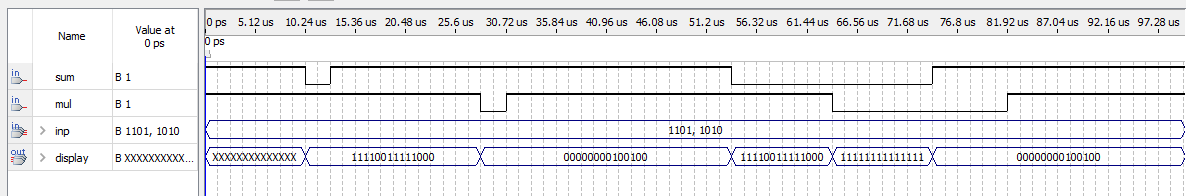
\includegraphics[width=1.4\textwidth]{analiza.png}
    \end{adjustwidth}
\end{figure}

Poniżej kod w języku VHDL:

\begin{figure}[H]
\begin{adjustwidth}{-1.3in}{-.7in} 
\centering
\begin{minted}{vhdl}
library ieee;
use ieee.std_logic_1164.all;
use ieee.numeric_std.all;

entity simple_calculator is
    port(
        a, b: in std_logic_vector(3 downto 0);
        sum, mul: in std_logic;
        display : out std_logic_vector(13 downto 0) := b"11111111111111"
    );
end simple_calculator;

architecture arch of simple_calculator is
    signal operation_result : std_logic_vector(7 downto 0);
    signal if_sum : std_logic := '0';
    signal if_mul : std_logic := '0';

    -- converts 4 bit unsinged number to states of 7 segment display in HEX
    function binary_to_ssd (
        switch : std_logic_vector(3 downto 0)
        )
        return std_logic_vector is variable sevenSegment : std_logic_vector(6 downto 0);
    begin 
        case switch is 
            -- 0 = display & 1 = no display
            when "0000" => sevenSegment := "1000000"; -- 0, 
            when "0001" => sevenSegment := "1111001"; -- 1
            when "0010" => sevenSegment := "0100100"; -- 2
            when "0011" => sevenSegment := "0110000"; -- 3 
            when "0100" => sevenSegment := "0011001"; -- 4
            when "0101" => sevenSegment := "0010010"; -- 5
            when "0110" => sevenSegment := "0000010"; -- 6
            when "0111" => sevenSegment := "1111000"; -- 7
            when "1000" => sevenSegment := "0000000"; -- 8
            when "1001" => sevenSegment := "0010000"; -- 9
            when "1010" => sevenSegment := "0001000"; -- A
            when "1011" => sevenSegment := "0000011"; -- b
            when "1100" => sevenSegment := "1000110"; -- C
            when "1101" => sevenSegment := "0100001"; -- d
            when "1110" => sevenSegment := "0000110"; -- E
            when others => sevenSegment := "0001110"; -- F
        end case;
        return sevenSegment;
    end binary_to_ssd;
\end{minted}
\end{adjustwidth}
\end{figure}

\begin{figure}
\begin{adjustwidth}{-1.3in}{-.7in} 
\centering
\begin{minted}{vhdl}
    -- converts 8 bit number to states of dual 7 segment display in HEX
    procedure display_value(value : std_logic_vector(7 downto 0)) is
    begin
        if value = b"11111111" then
            display <= b"11111111111111";
        else
            display <= binary_to_ssd(value(7 downto 4)) & binary_to_ssd(value(3 downto 0));
        end if;
    end procedure display_value;
    
begin
    process(sum, mul)
    begin
        if sum = '0' and mul = '0' then
            if_mul <= '0';
            if_sum <= '0';
        elsif sum = '0' then
            if_sum <= '1';
            if_mul <= '0';
        elsif mul = '0' then
            if_mul <= '1';
            if_sum <= '0';
        end if;
    end process;

    operation_result <= 
        std_logic_vector(resize(unsigned(a), operation_result'length) + unsigned(b)) when if_sum = '1' else
        std_logic_vector(unsigned(a) * unsigned(b)) when if_mul = '1' else
        b"11111111";
    
    display_value(operation_result);
    
end arch;

\end{minted}
\end{adjustwidth}
\end{figure}

\end{document}